\documentclass[10pt]{article}
\usepackage[utf8]{inputenc}
\usepackage[english]{babel}
\usepackage[font=small,labelfont=bf]{caption}
\usepackage{geometry}
\usepackage[sort&compress, numbers]{natbib}
\usepackage{pxfonts}
\usepackage{graphicx}
\usepackage{setspace}
\usepackage{hyperref}
\usepackage{lineno}

\newcommand{\demo}{S1}

\doublespacing
\linenumbers

\title{Geometric models reveal the hidden structure of conceptual knowledge}

\author{Paxton C. Fitzpatrick\textsuperscript{1} and Jeremy R.
Manning\textsuperscript{*, 1}\\\textsuperscript{1}Dartmouth
College\\\textsuperscript{*}Corresponding author:
jeremy.r.manning@dartmouth.edu}

\date{}

\begin{document}
\maketitle

\begin{abstract} We develop a mathematical framework, based on natural language
processing models, for tracking and characterizing the acquisition of
conceptual knowledge. Our approach embeds each concept in a high dimensional
representation space, where nearby coordinates reflect similar or related
concepts. We tested our approach using behavioral data collected from a group
of college students. In the experiment, we asked the participants to answer
sets of quiz questions interleaved between watching two course videos from the
Khan Academy platform. We applied our framework to the videos' transcripts, and
to text of the quiz questions, to quantify the content of each moment of video
and each quiz question. We used these embeddings, along with participants' quiz
responses, to track how the learners' knowledge changed after watching each
video. Our findings show how a limited set of quiz questions may be used to
construct rich and meaningful representations of what each learner knows, and
how their knowledge changes over time as they learn.

\textbf{Keywords: education, learning, knowledge, concepts, natural language processing}

\end{abstract}


\section*{Main text}

\begin{figure}[tp]
\centering
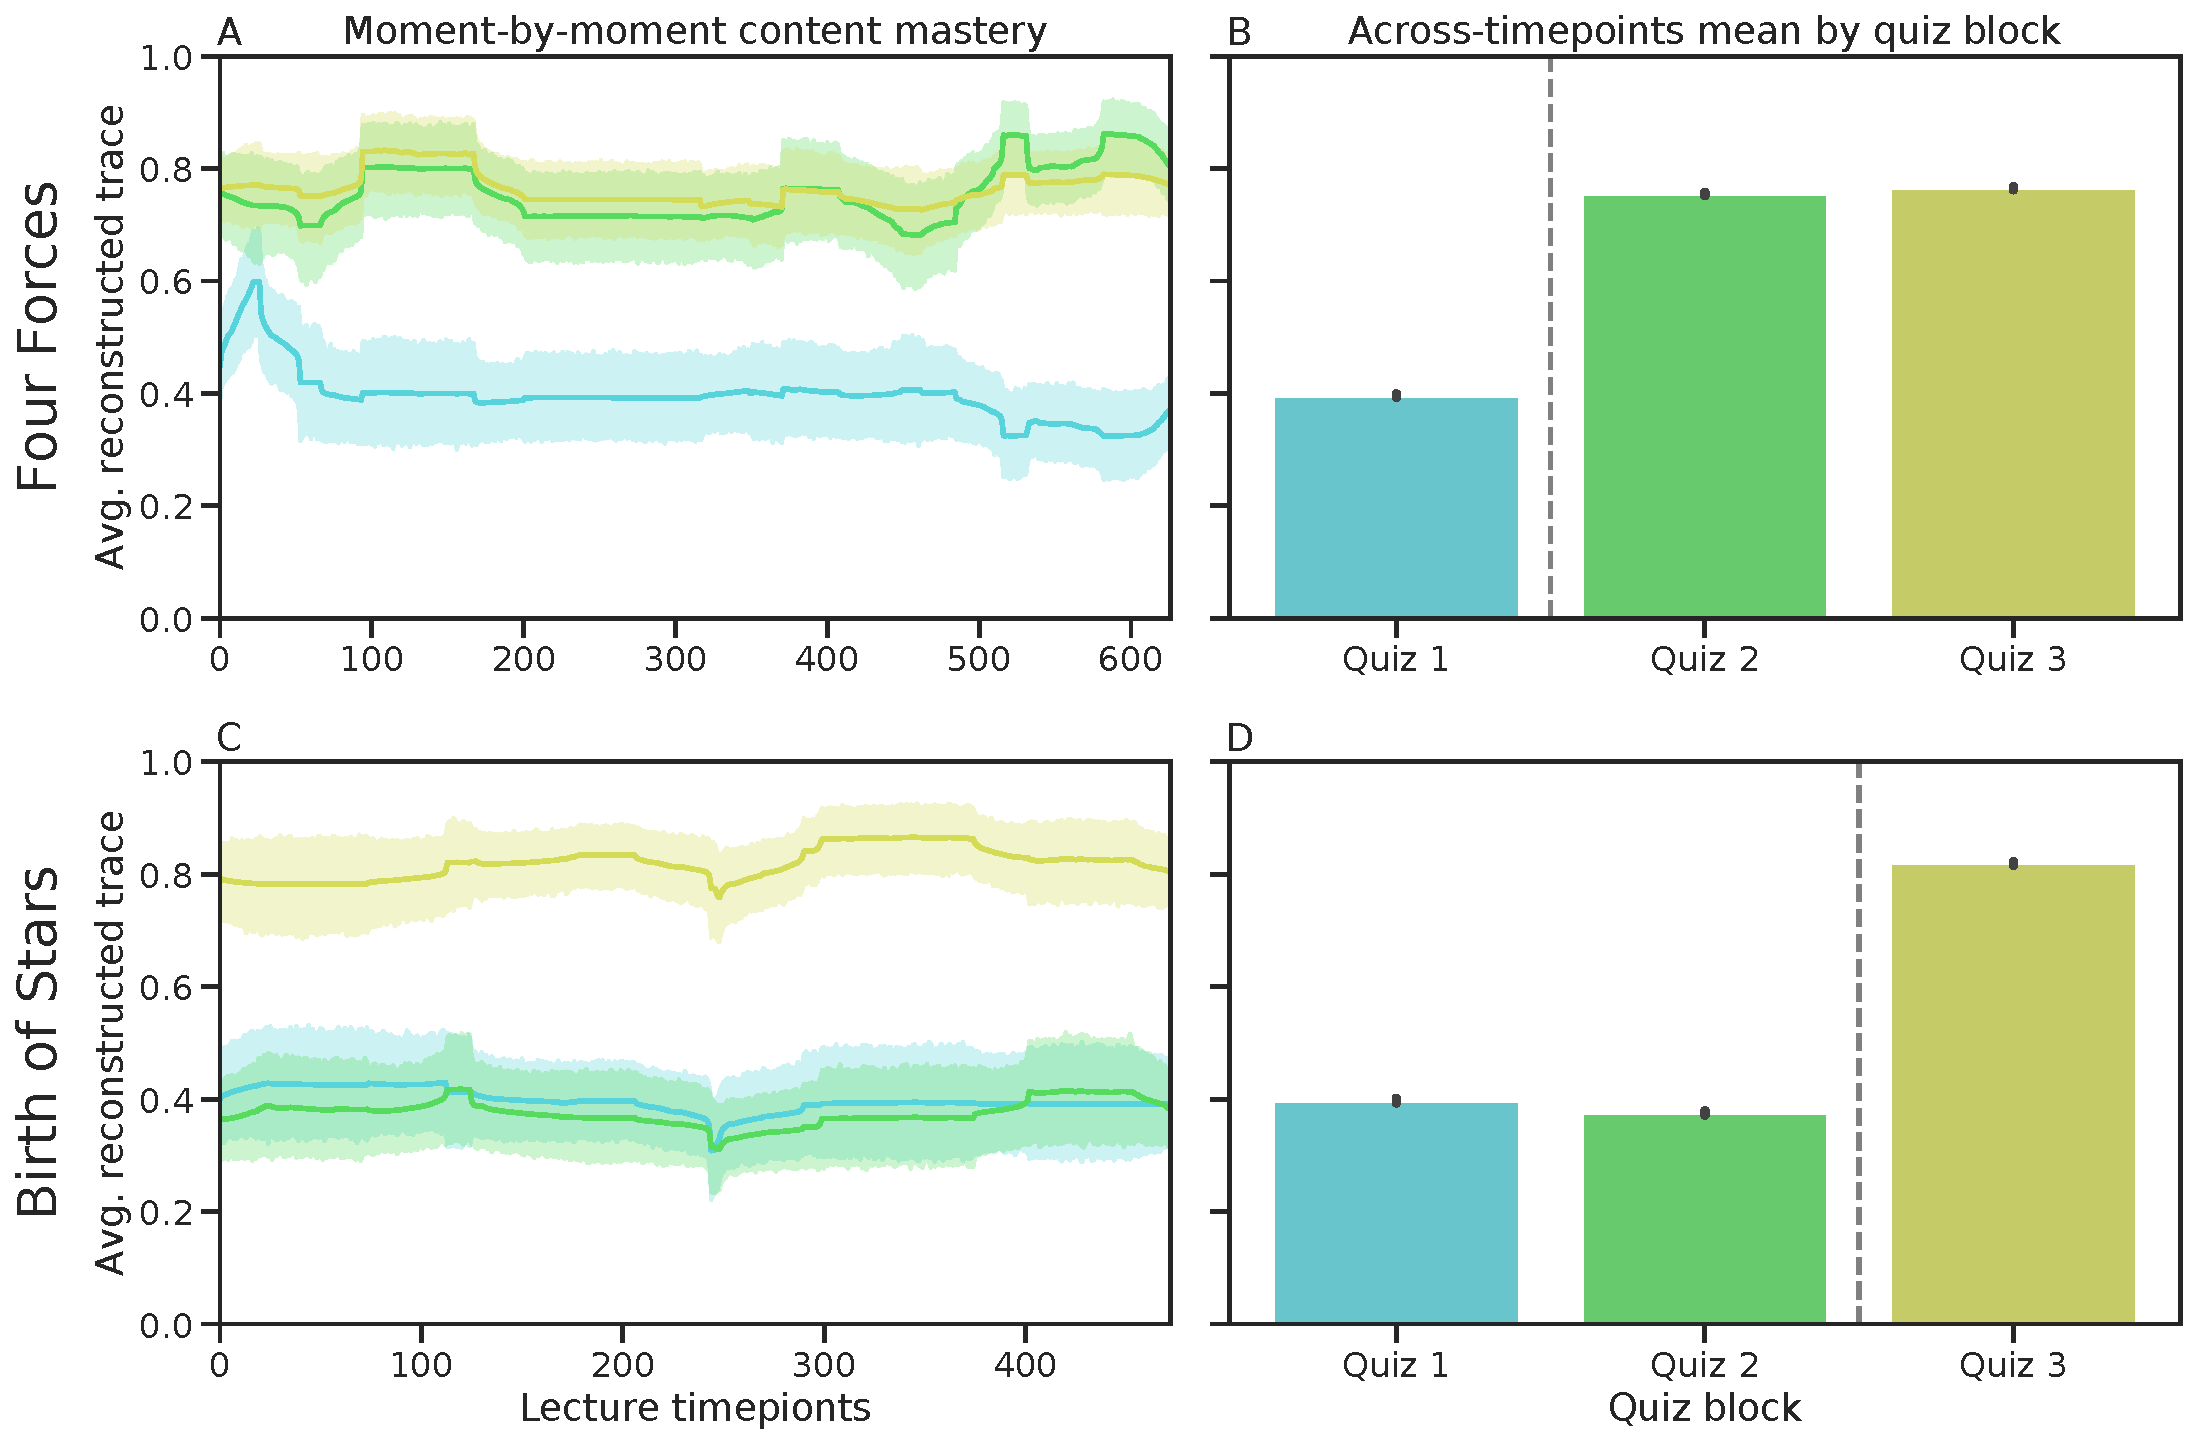
\includegraphics[width=0.8\textwidth]{figs/content-mastery}
\caption{\textbf{Caption.} Placeholder text.}
\label{fig:demo}
\end{figure}

Insert text here (Figs.~\ref{fig:demo}, \demo).

\bibliographystyle{apa}
\bibliography{CDL-bibliography/cdl}
\end{document}
